In this section, we describe how the module designs detailed in
\autoref{sec:design} are implemented on a Xilinx Virtex4
XC4VFX12-SF363-12 FPGA. The implementation description is based on the
synthesis results from using the XST synthesiser from the ISE design
suite WebPACK Edition. The modules are not represented as separate
VHDL files or entities, but are only a conceptual model of how the
system works.

\subsection{Technology Schematic}
\label{sec:technologyschematic}

\autoref{fig:technologyschematic} shows how each functionality
of the Liaison from \autoref{fig:overview} is mapped to the LUTs in
the syntesised design.  Each functionality are marked with a distinct
colour. Note that LUTs marked as either ``Status Calculation'' or
``State Maintenance'' functionality are both a part of the State
Maintenance module.


\begin{figure}[p]
  \vspace*{-1.2in}
  \centerline{ 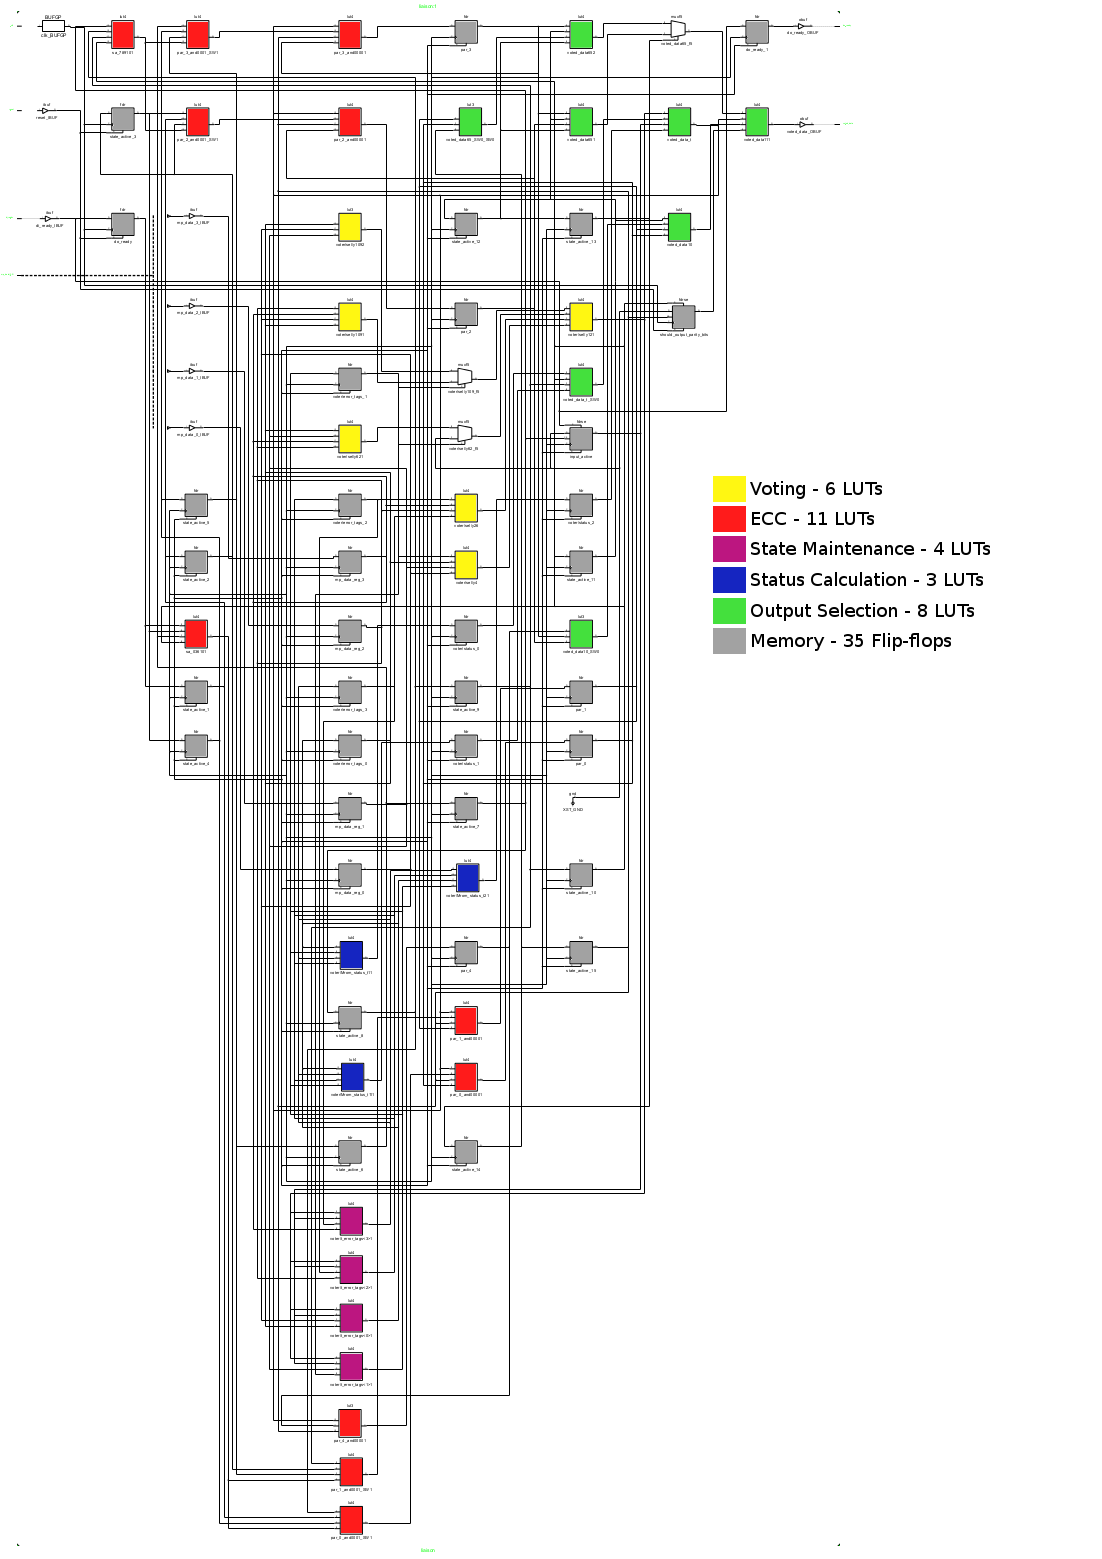
\includegraphics[width=1.2\textwidth]{LUT-count} }
  \caption{The technology schematic of our Liaison}
  \label{fig:technologyschematic}
\end{figure}

\subsection{Voting Algorithm Implementation}
The implementation of our voting algorithm, described in
\autoref{sec:votingalgorithm}, consists of six LUTs and two MUXes. In
the implementation, microcontroller 0, 1, 2 and 3 maps to the labels
A, B, C and D in the design description. The input microcontroller
data is combined with the error tags according to the algorithm,
emitting the result of the (A,~B) local vote if this is safe to use,
the (C,~D) result if this is safe, and the ORed result in other cases.

%NO NO NO red.anm.
%It is impossible for man to figure out what the hell these LUTs
%do... they certainly do not match the VHDL code.

\subsection{State Maintenance Implementation}
\label{sec:statemaintenance}
The state maintenance is implemented with a number of registers, and
the required logic for updating each of them.

Since we send 16 bits per voted word, the output stage state is
represented by 16 flip-flops connected in sequence, implementing a
shift-register. These registers will be referred to as output stage
bits 1 to 16. 

To update the error tags only during microcontroller data word
transmission states, we need to produce an enable signal. This signal
is implemented with a flip-flop which is set when di\_ready is set,
and cleared when output stage bit 8 is set. Since the update occurs at
the start of each clock cycle, and the enable signal is only set on
the start of the output stage, we have to use flip-flops to keep the
input data stable throughout the next clock period. If, instead, the
output signals were kept stable with flip-flops, the error tags
calculated from the first data bit would be lost since the enable
signal would not have been set when they were calculated. Thus, we
also use four flip-flops to contain the microcontroller data.

The error tags are implemented with four flip-flops. To update the
error tags, one LUT is used to calculate the new value of each flip
flop. These LUTs take as input the old error tag value, the
microcontroller data, the result of the vote and the enable
signal.  If the old error tag
was set, the new error tag is also set. Else, if the enable signal is
high, the error tag is set if the microcontroller data differs from
the voted data.

The status bits are calculated based on the error tags. Since there
are only four error tags, we can calculate each status bit with one
LUT each, so the status calculation is implemented with 3 LUTs. 

The state also includes five parity bit registers, whose update
semantics will be explained in in \autoref{sec:eccimplementation}.

\subsection{Error Correction Code Implementation}
\label{sec:eccimplementation}
The implementation of the error correction code calculation is
illustrated in \autoref{fig:ecc}. 

\begin{figure}
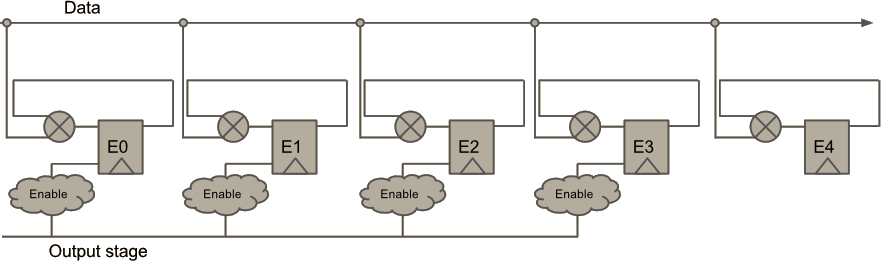
\includegraphics[width=15cm]{implementation/fig_ecc}
\caption{Implementation of Hamming(16,11)}
\label{fig:ecc}
\end{figure}

Apart from the SECDED bit, each parity bit calculates the parity over
some subset of data bits. Since the data is computed sequentially and
the parity bits are computed on the fly as the data is being sent, it
is necessary to implement some control logic for each parity bit to
determine whether the current data bit being sent is one the parity
bit is supposed to cover or not. This control logic is depicted as the
\textit{Enable} clouds in \autoref{fig:ecc}. Since the SECDED bit is
supposed to cover all the bits, it does not need this enable signal. 

For each parity bit, there is a LUT computing its next value. This LUT
takes as input the current data, the previous value of the parity bit,
and the final output stage bit. For the ECC bits apart from the SECDED
bit, there is also a signal stating whether the current data bit is
one the parity bit covers or not. If we are in the final output stage,
the parity bit is reset to 0 to reset the count for the next data
word. If the parity bit is supposed to cover the current data bit, the
next parity bit value is the XOR of the data bit and the previous
parity bit value. If not, the parity bit value is kept as is. 

Since the subsets of data bits covered for each parity bit partially
overlap, it is possible to compute parts of differerent enable signals
with the same LUT. For instance, parity bit number 2 and 3 both cover
data bits 7, 8, 9 and 10. Since the enable signal is computed using an
OR of the relevant output stage bits, a single LUT for computing the
OR between output stage bit 7, 8, 9 and 10 is needed. The independent
enable signal for parity bit 2 and 3 can then be computed by ORing the
output of this LUT with the three remaining output stage bits. Thus,
six LUTs are required to compute the different enable signals, and
with one LUT for each parity bit to update its value eleven LUTs are
used in total.

\subsection{Output Selection Implementation}
The output selection determines which of the candidate output bits ---
voted data, a status bit or an ECC bit --- should be output next. This
selection is performed in several stages. 

One stage chooses between the voted data bit and the status bits. One
LUT is used to compute which of the two least significant status bits
if any should be output, and 0 otherwise. Then, a second LUT combines
this bit with the voted data bit, the most significant status bit, and
a signal stating whether we should send a data bit or not. This signal
is the output of a register which is set at the same time as output
stage bit 1, and cleared when output stage bit 9 is set. If the signal
is 1, then the output of the LUT is the voted data. If not, the output
is the most significant status bit ORed with the selection of the two
least significant status bit. Since the most significant status bit is
set implies the two least significant status bit being set, this OR
will not pollute the least significant status bit, and make sure the
most significant bit is sent at its time.

To compute the error correction code bit, the SECDED bit is computed
by XORing the ECC flip-flop values. The ECC bit is selected by
combining the last output stage bits. Finally, the data output is
selected between the ECC bit and the data-status bit based on a signal
stating whether we should output an ECC bit or not. This signal is
also the output of a flip-flop, set and cleared based on output stage
bits. This step requires seven LUTs and one MUX, and the total LUT
count for the output multiplexing is eight LUTs.

\subsection{Results}

The main metrics of our system is given in
\autoref{tab:results}. Metrics found with two different synthesis
tools are shown.

\begin{table}[htbp]
  \centering
  \begin{tabular}{|c|c|c|}
    \hline
    \textbf{Metric} & XST Synthesiser Results & Synplify Pro Results \\ \hline
    Number of LUTs & 32 & 37 \\ \hline
    Number of flip-flops & 35 & 34 \\ \hline
    Estimated clock frequency & 318.715 MHz & 322 MHz \\ \hline
  \end{tabular}
  \caption{System Results}
  \label{tab:results}
\end{table}
